\documentclass{IEEEtran}  
\usepackage{amsmath}
\usepackage{graphicx}
\usepackage[font=small,labelfont=bf]{caption}
\DeclareCaptionType{copyrightbox}
\usepackage{subcaption}
\usepackage{amssymb}
\usepackage{amsfonts}
\usepackage{authblk}
\usepackage{url}
\usepackage{color}
\usepackage[lined, boxed]{algorithm2e}
\usepackage{colortbl}
\definecolor{Gray}{gray}{0.85}

\newcommand{\er}{Erd\H{o}s-R\'{e}nyi } 
\newtheorem{thm}{Theorem}
\newtheorem{cor}{Corollary}
\newtheorem{defn}{Definition}
\newtheorem{propn}{Proposition}
\newtheorem{obs}{Observation}

\begin{document}

\title{Locally Boosted Graph Aggregation and Community Detection}

%\thanks{This
%work is sponsored by the Assistant Secretary of Defense for Research \&
%Engineering under Air Force Contract FA8721-05-C-0002.  Opinions,
%interpretations, conclusions and recommendations are those of the authors and
%are not necessarily endorsed by the United States Government.}}
\author[]{Submitted for blind review}
%\author[1,2]{Jeremy Kun}%\thanks{jkun2@uic.edu}} 
%\author[1]{Rajmonda S. Caceres}%\thanks{rajmonda.caceres@ll.mit.edu}}
%\author[1]{Kevin M. Carter}%\thanks{kevin.carter@ll.mit.edu}}
%\affil[1]{MIT Lincoln Laboratory}
%\affil[2]{University of Illinois at Chicago}


\date{}

\maketitle

\begin{abstract} \small \baselineskip=9pt 
Learning the right graph representation from noisy, multi-source data has
garnered significant interest in recent years. A central tenet of this problem
is relational learning. Here the objective is to incorporate the partial
information each data source gives us in a way that captures the true
underlying relationships. To address this challenge, we present a general,
boosting-inspired framework for combining weak evidence of entity associations
into a robust similarity metric. We explore the extent to which different local
quality measurements yield graph representations that are suitable for
community detection. We present empirical results on a variety of datasets
demonstrating the utility of this framework, especially with respect to real
datasets where noise and scale present serious challenges. Finally, we prove a
convergence theorem and outline future research into other application domains.
\end{abstract}
 
\section{Introduction}

When studying networks, the data used to define nodes and edges often come from
multiple sources. These sources can be noisy and ambiguously useful, and the
process of combining them into a single graph representation is critically
important. For example, when studying communities in social networks the data
that indicate membership in the same community are plentiful: communication,
physical proximity, reported friendship, etc. Each data source carries 
different information about the underlying social structure, and each
may accurately represent only some of the individuals. Some groups of friends
communicate through Facebook and others via Instagram, etc. The best way to
aggregate this information is unclear, and the choice of graph
representation significantly impacts the performance of subsequent data mining
algorithms \cite{Getoor2005,Gallagher2008,Neville2005,Caceres2011,Miller2014}.
Further complicating matters, the quality of the aggregated graph depends on
the application domain. Community detection is easiest with a graph
representation that discards cross-community edges, but to predict the
spread of a virus one must keep crucial cross-community conduits. Suitable
graph representations for these tasks may use the same data but are different
enough to need different aggregation techniques. 

Even though the impact of the graph representation on subsequent analysis has
been widely studied, there are few techniques for learning good graph
representations. Aggregation is often ad-hoc in practice, making it difficult
to compare algorithms within the same domain using different data sources. The
need for rigorous approaches to graph representation learning is even more
apparent with big data.

In this paper, we present a graph aggregation framework designed to make the
process of learning a useful underlying graph representation rigorous with
respect to application specific requirements. Our framework is called
\emph{Locally Boosted Graph Aggregation (LBGA)}. LBGA extracts the
application-specific aspects of the learning objective as an event $A$
representing an operation on the graph (e.g. a clustering algorithm, a random
walk, etc.) and a local quality measure $q$. Using these, the framework
simulates a reward system that promotes the presence of good edges and the
absence of bad edges, in a fashion inspired by boosting.

%Building on~\cite{CCK14}, 
We demonstrate LBGA applied to community detection.  In this context the goal
of graph representation learning is to aggregate the different data sources
into a single graph which makes the true community structure easy to detect.
LBGA evaluates the graph data locally, so that it can choose the data sources
which most accurately represent the local structure of communities observed in
real networks~\cite{Aggarwal2011,Leskovec2008}. In the absence of ground truth
knowledge or one efficiently computable measure that can capture true community
quality, LBGA relies on the pair of a graph clustering algorithm $A$ and a
local clustering metric $q$ as an evaluation proxy.  We show through empirical
analysis that our algorithm can learn a high-quality global representation
guided by the local quality measures considered. 

We make the following contributions:

\begin{enumerate} 
   \item We present a graph aggregation framework that learns a useful graph
representation with respect to an application requiring only a local heuristic
measure of quality.
   \item Our framework is stochastic and incorporates both edge and non-edge
information, making it robust and suitable for sparse and noisy networks.
   \item We demonstrate the success of an algorithm implementing the framework
for community detection, testing it against both synthetic data and real-world
data sets. 
   \item We perform sensitivity and scalability analyses of our algorithm,
showing that the algorithm scales linearly in the number of edges and is
robust enough to handle large, noisy graphs.  
   \item We prove a convergence theorem for our framework and suggest the next
steps in proving performance guarantees.  
\end{enumerate} 

We emphasize that while this paper specifically addresses community detection,
the central focus here is on aggregating multiple noisy, potentially
adversarial graphs into a single graph. Even though the definition of what
makes an edge qualitative depends on the application, the core piece of our
algorithm, the edge reward mechanism and the graph aggregation step, are
application agnostic. 
%Because the ``correct'' graph aggregation depends on the application, our core
%algorithm is application agnostic.  Moreover, standard clustering algorithms
%do not apply to our setting because they operate on a single graph.

This paper is organized as follows. In Section~\ref{sec:related} we review
related literature. In Section~\ref{sec:lbga} we discuss in detail the LBGA
framework. In Section~\ref{sec:experiments} we present the experimental
analysis and results. In Section~\ref{sec:additional-analysis} we discuss
sensitivity to noise and scalability. In Section~\ref{sec:convergence-theorem}
we prove our convergence theorem, and in Section~\ref{sec:conclusion} we
discuss future work.

\section{Related work} 
\label{sec:related}
\subsection{Representation learning and clustering}
Representation learning has garnered a lot of interest and research in recent
years. Its goal is to introduce more rigor to the often ad-hoc practices of
transforming raw, noisy, multi-source data into inputs for data mining and
machine learning algorithms. Within this area, representation learning of
graph-based data includes modeling decisions about the nodes of the graph, the
edges, as well as the critical features that characterize them both.

In this context, Rossi et al.~\cite{Rossi2012} discuss transformations to
heterogeneous graphs (graphs with multiple node types and/or multiple edge
types) in order to improve the quality of a learning algorithm. Within their
taxonomy, our work falls under the link interpretation and link re-weighting
algorithms \cite{Xiang2010,Gilbert2009}. Our setting is different because we
explicitly allow different edge types between the same pair of vertices. Also,
our approach is stochastic, which we find necessary for learning a robust
representation and weeding out noise. 

Clustering in multi-edge graphs
\cite{Papalexakis2013,Tang2009,Tang2012,Mucha2010,Berlingerio2011,kolda2009} is
another area with close connections to our work. A common thread among these
existing approaches is clustering by leveraging shared information across
different graph representations of the same data. These approaches do not
address scenarios where the information provided by the different sources is
complementary or the overlap is scarce. In contrast, our approach iteratively
selects those edge sources that lead to better clustering quality,
independently of disagreement across the different features.
\cite{Rocklin2013,Cai2005} present approaches for identifying the right graph
aggregation, given a complete ground truth clustering, or a portion of it
(i.e.: the cluster assignment is known only for a subset of the vertices in the
graph). Our framework requires no such knowledge, but we do use ground truth to
validate our experiments on synthetic data (Section \ref{sec:validation}).
Balcan and Blum define in \cite{Balcan2006,Balcan2008} a list of intuitive
properties a similarity function needs to have in order to be able to cluster
well. However, testing whether a similarity function has the discussed
properties is NP-hard, and often dependent on having ground truth available.
Our model instead uses an efficiently computable heuristic as a rough guide.

\subsection{Boosting and bandits}
Our framework departs from previous work most visibly through its algorithmic
inspirations, namely boosting \cite{Schapire90} and bandit learning
\cite{Bubeck12}. Neither framework applies directly to our problem, but they
suggest a natural algorithm whose simplifications have measurable convergence
properties. 

In boosting, one assumes the existence of a {\em weak classifier} whose
performance is slightly better than random. In a landmark paper
\cite{Schapire90}, Schapire showed how to combine weak classifiers into a
PAC-learner by a majority voting scheme. One can consider different graph data
sources as weak learners, and ask whether one can ``boost'' them to a good
graph. Unfortunately, our problem setting does not allow pure boosting for two
reasons: input graphs can be pure noise or adversarially bad and hence are not
weak learners; and boosting requires access to ground truth labels. Even with
reliable input, the application domain may have no accepted measure of quality. 

Ideas from bandit learning compensate for these problems. In bandit learning an
algorithm receives rewards as it explores a set of actions, and the goal is to
minimize some notion of regret in hindsight. The basic model has many variants,
but two central extensions in the literature are expert advice and adversaries.
Experts are functions suggesting what action to take in each round (which are
arbitrary). The adversarial setting involves an omniscient adversary who sets
the experts and rewards so as to maximize regret. In particular, rewards can
vary across rounds.

Using these ideas, we set up a reward system based on the given application and
use stochastic weight update techniques to learn a graph representation. In our
setting we only care if the aggregate graph is good at the end, while bandit
learning often seeks to maximize cumulative rewards during learning. There are
bandit settings that only care about the final result (e.g., pure exploration
\cite{Bubeck09}), but to the best of our knowledge they do not apply to our
problem. 

The primary technique we adapt from bandits and boosting is the
Multiplicative Weights Update Algorithm (MWUA). See \cite{Arora12} for an
overview and an extensive list of successful applications. The algorithm
maintains a weight for each element $x_j$ of a finite set $X$. In rounds,  
an element $x_i$ is chosen by sampling proportionally to the weights, a reward
$q_{t,i}$ is received, and the weight for $x_i$ is multiplied or divided by $(1
+ \varepsilon q_{t,i})$, for some parameter $\varepsilon >0$. After many
rounds, the elements with the highest weight are deemed the best and used for
whatever purpose needed. Next, we describe how this algorithm is adapted to
graph aggregation. 

\section{The Locally Boosted Graph Aggregation framework}
\label{sec:lbga}

The Locally Boosted Graph Aggregation framework (LBGA) can succinctly be
described as running MWUA for each possible edge, forming a candidate graph
representation $G_t$ in each round by sampling from all edge distributions, and
computing local rewards on $G_t$ to update the weights for the next round. Over
time $G_t$ stabilizes and we produce it as output. The remainder of this
section expands the details of this sketch and our specific algorithm
implementing it.  

\subsection{Framework details}
\label{sec:framework}

Let $H_1, \dots, H_m$ be a set of unweighted, undirected graphs defined on the
same vertex set $V$. We think of each $H_i$ as ``expert advice'' suggesting for
a pair of vertices $u,v \in V$ whether to include edge $(u,v)$ or not. Our goal
is to combine the information present in the $H_i$ to produce a global graph
representation $G^*$ suitable for a given application. 

We present LBGA in the context of community detection, noting generalizations.
Each round has four parts: producing the aggregate candidate graph $G_t$,
computing a clustering $A$ for use in measuring the quality of $G_t$, computing
the local quality of each edge, and using the quality values to update the
weights for the edges. After some number of rounds $T$, the process ends and we
produce $G^* = G_T$.

\textbf{Aggregated Candidate Graph $G_t$}: In each round produce a graph $G_t$
as follows. Maintain a weight $w_{u,v,i}$ for each graph $H_i$ and each edge
$(u,v)$ in $H_1 \cup \dots \cup H_m$. Normalize the set of all weights for an
edge $\mathbf{w}_{u,v}$ to a probability distribution over the $H_i$; thus one
can sample an $H_i$ proportionally to its weight. For each edge, sample in this
way and include the edge in $G_t$ if it is present in the drawn $H_i$. 

\textbf{Event $A(G_t)$}: After the graph $G_t$ is produced, run a clustering
algorithm $A$ on it to produce a clustering $A(G_t)$. In this paper we fix $A$
to be the Walktrap algorithm \cite{Walktrap}, though we have observed the
effectiveness of other clustering algorithms as well. In general $A$ can be any
event, and in this case we tie it to the application by making it a simple
clustering algorithm.

\textbf{Local quality measure}: Define a \emph{local quality measure}
$q(G,e,c)$ to be a $[0,1]$-valued function of a graph $G$, an edge $e$ of $G$,
and a clustering $c$ of the vertices of G. The quality of $(u,v)$ in $G_t$ is
the ``reward'' for that edge, and it is used to update the weights of each
input graph $H_i$.  More precisely, the reward for $(u,v)$ in round $t$ is
$q(G_t, (u,v),A(G_t))$.

\textbf{Update Rule}: Update the weights using MWUA as follows. Define two
learning rate parameters $\varepsilon > 0, \nu > 0$, with the former being used
to update edges from $G_t$ that are present in $H_i$ and the latter for edges
not in $H_i$. In particular, suppose $q_{u,v}$ is the quality of the edge
$(u,v)$ in $G_t$. Then, the update rule is defined as follows:
\[
w_{u,v,i}=
\begin{cases}
w_{u,v,i}(1 +\varepsilon q_{u,v}), & \text{if } (u,v) \in H_i \\
w_{u,v,i}(1 - \nu q_{u,v}), & \text{if } (u,v) \not \in H_i .
\end{cases}
\]
 
\subsection{Quality measures for community detection}
\label{sec:quality-measures}
We presently describe the two local quality measures we use for community
detection. The first, which we call {\em Edge Consistency} ($EC$) asserts that
edges with endpoints in the same cluster are superior to edges across clusters:
\[
   EC_{u,v}=
   \begin{cases}
   1, & \text{if  }c(u) = c(v) \\
   -1,  & \text{if  }c(u) \neq c(v).
   \end{cases}
\]
$EC$ offers a quality metric that is inextricably tied to the performance of
the chosen clustering algorithm, and as such we have found it performs poorly
in practice. However, edge consistency can be combined with any quality
function $q$ to produce a ``consistent'' version of $q$. Simply evaluate $q$
when the edge is within a cluster, and $-q$ when the edge is across clusters.
Note that $q$ can represent an algorithmic-agnostic measure of clustering
quality. 

As an example, we define \emph{Neighborhood Overlap} ($NO$), which uses the
idea that vertices that share many neighbors are likely to be in the same
community. NO declares the quality of $(u,v)$ to be the (normalized)
cardinality of the intersection of the neighborhoods of $u$ and $v$, namely
$NO_{u,v}=\frac{|N(u) \cap N(v)|}{|N(u) \cap N(v)| + log(|V|)},$ where $N(x)$
represents the neighborhood of vertex $x$. We have also run experiments using
more conventional normalizing mechanisms, such as the Dice and Jaccard
indices~\cite{Dice1945,Jaccard1912}), but our neighborhood overlap metric
outperforms them by at least 10\% in our experiments. We argue this is due to
the use of a global normalization factor, as opposed to a local one, which is
what Dice and Jaccard indices use. For brevity and simplicity, we omit our
results for Jaccard and Dice indices and focus on Neighborhood Overlap. In our
experimental analysis (Section~\ref{sec:results}) we use the consistent version
of $NO$, which we denote \emph{consistentNO}. 

While we demonstrate the utility of the LBGA framework by using $consistentNO$,
the design of the framework is modular, in that the mechanism for rewarding the
``right'' edges is independent from the definition of reward. This allows us
to plug in other quality metrics to guide the graph representation learning
process for other applications.

Lastly, the quality of an edge is dictated by the choice of the clustering
algorithm (event). In our case, walktrap merges clusters with the objective of
maximizing modularity and this affects the presence of small clusters. To
alleviate this, one can use a modified walktrap that outputs similarity values,
or re-run LBGA on the graphs induced by the vertices belonging to the resulting
clusters. The latter gives a hierarchical clustering, and LBGA can identify
hierarchical community structure in this way, though we omit the details for
brevity. 

\subsection{LBGA implementation} 
Processing every edge in every round of the LBGA framework is inefficient.  Our
implementation of LBGA, given by Algorithm~\ref{alg:nef}, improves efficiency
by fixing edges whose weights have grown so extreme so as to be picked with
overwhelming or negligible probability (with probability $ > 1-\delta$ or $<
\delta$ for a new parameter $\delta$). In practice this produces a dramatic
speedup on the total runtime of the algorithm, because as the algorithm learns
the sampling procedure becomes substantially sublinear in the number of
edges. The worst-case time complexity is the same, but we discuss practical
methods to speed up LBGA in Section~\ref{sec:scalability-analysis}. 

In addition, our decision to penalize non-edges ($\nu > 0$) also improves
runtime from the alternative ($\nu = 0)$. In our experiments non-edge feedback
causes $G_t$ to convergence in roughly half as many rounds as when only
presence of edge is considered as indication of relational structure. Moreover,
the algorithm is stable to minor variations in $\varepsilon$ and $\delta$.
Indeed, the theoretical guarantees of MWUA in general and
Section~\ref{sec:convergence-theorem} suggest that for any fixed $0 < \varepsilon,
\delta < 1/2$ the algorithm converges in at most $O(\log(n/\delta))$ rounds.

We also note that Algorithm \ref{alg:nef} stays inside the ``boundaries''
determined by the input graphs $H_i$.  It never considers edges that are not
suggested by \emph{some} $H_i$, nor does it reject an edge suggest by all
$H_i$. Thus, when we discuss sparsity of our algorithm's output in our
experiments, we mean with respect to the number of edges in the union of the
input graphs.

\begin{algorithm}[tbh]
\caption{Optimized implementation of LBGA. Note that $1_E$ denotes the
characteristic function of the event $E$.}
\label{alg:nef}
   \DontPrintSemicolon
   \SetAlgoLined
   {\footnotesize
   \KwData{Unweighted graphs $H_1, \dots, H_m$ on the same vertex set $V$, a
clustering algorithm $A$, a local quality metric $q$, three parameters
$0 < \varepsilon, \nu, \delta < 1/2$}
   \KwResult{A graph $G$}
   Initialize a vector $\mathbf{w}_{u,v} = \mathbf{1}$ for all $u \neq v \in V$\;
   Let $U$ be the edge set of $H_1 \cup \dots \cup H_m$\;
   Let $G_\textup{learned} = (V, \varnothing)$ \;
   \While{$|U| > 0$}{
      Let $G$ be a copy of $G_{\textup{learned}}$\;

      \For{$(u,v) \in U$}{
         Let $p_{u,v} = \frac{\sum_i w_{u,v,i} 1_{\left \{(u,v) \in H_i \right \}}}{\sum_i w_{u,v,i}}$ \;
         Flip a coin with bias $p_{u,v}$\;
         If heads, include $(u,v)$ in $G$.
      }

      Cluster $G$ using $A$\;

      \For{$(u,v) \in U$}{
         Set $p = q(G, A(G), (u,v))$\;
         \For{$i = 1, \dots, m$}{
            \eIf{$(u,v) \in H_i$}{
               Set $w_{u,v,i} = w_{u,v,i} (1 + \varepsilon p)$\;
            } {
               Set $w_{u,v,i} = w_{u,v,i} (1 - \nu p)$\;
            }
         }

         Let $p_{u,v} = \frac{\sum_i w_{u,v,i} 1_{\left \{(u,v) \in H_i \right \}}}{\sum_i w_{u,v,i}}$ \;
         \If{$p_{u,v} > 1-\delta$}{
            Add $(u,v)$ to $G_{\textup{learned}}$, remove it from $U$\;
         }
         \If{$p_{u,v} < \delta$}{
            Remove $(u,v)$ from $U$\;
         }
      }
   }
   Output $G$\;
}
\end{algorithm}

\section{Experimental analysis}
\label{sec:experiments}
We describe the datasets used for analysis and provide quantitative results for
the performance of Algorithm \ref{alg:nef}. 

\subsection{Synthetic datasets}
\label{sec:synthetic-model}

Our primary synthetic data model is the stochastic block model \cite{Wang87},
commonly used to model explicit community structure.  We construct a
probability distribution $G(\mathbf{n},B)$ over graphs as follows. Given a
number $n$ of vertices and a list of cluster (block) sizes $\mathbf{n}=\{n_1,
\dots, n_k\}$ such that $n =\sum_i n_i$, we partition the $n$ vertices into $k$
blocks $\{b_1, \dots, b_k\}$, $|b_i|=n_i$.  We declare that the probability of
an edge occurring between a vertex in block $b_i$ and block $b_j$ is given by
the $(i,j)$ entry of a $k$-by-$k$ matrix $B$. 

A reformulation of the stochastic block model in the multimodal setting
considers how strongly each graph source represents each community in data. In
the most local case, each graph source represents well only one community. We
can model this as follows. Fix some probability $p_i$ of an edge occurring within
a community and $r_i$ for an edge occurring across communities ($p_i>>r_i$). Then
draw the input graph $H_i$ from the distribution $G(\mathbf{n}, B_i)$, where
$B_i$ has $p_i$ in its $(i,i)$ entry and $r_i$ everywhere else. For example, if
there are $m=2$ communities the probability matrices would be
\[
B_1=\begin{pmatrix}
p_1 & r_1 \\
r_1 & r_1
\end{pmatrix},
\hspace{0.5cm}
B_2=\begin{pmatrix}
r_2 & r_2 \\
r_2 & p_2
\end{pmatrix}
.\]
We call this model the \emph{local stochastic block model} (LSBM).  We can
further vary the number of communities each graph source strongly represents,
with the other extreme being the case where each graph source has a global
contribution toward the overall community structure. We refer to this case as
the \emph{global stochastic block model} (GSBM).

Finally, we consider the case of the \emph{\er random graph}~\cite{Erdos60},
where any two vertices have equal probability of being connected. This model
provides an example of a graph with no community structure. Note that the ER
model is a special case of LSBM with $p=r$. We also consider cases where an ER
model is injected into block model instances in order to capture a range of
structure and noise combinations.

\begin{table}
\begin{tabular}{| l | l |}
\hline
Dataset & Parameters\\
\hline \hline
GSBM-4 & $m =k= 4, n_i=125, p_1=0.1625, $ \\ 
       & $p_2 = 0.125, p_3 = 0.125, p_4 = 0.0875, r_i = 0.05$ \\
       
GSBM-5 & $m=k=4, n_i=125, p_1=0.15, p_2=0.1,$ \\ 
       & $p_3=p_4=0.05, r_i = 0.05, i=1, \ldots, m$ \\

\hline
LSBM-1 & $m=k=4, n_i=125, p_i=0.2, r_i=0.05$ \\
LSBM-2 & $m=k=4, n_i=125, p_i=0.3, r_i=0.05$ \\
LSBM-3 & $m=5,k=4, n_i=125, p_i=0.3, r_i=0.05$, \\ 
       & $i = 1, \dots, m, p_5= r_5 = 0.01$ \\
\hline
ER only &  $m=4, p_i=r_i=0.01$ \\
DBLP    & $n = 3153, m = 2$ \\
RealityMining      & $n = 90, m = 6$ \\
Enron   & $n = 145, m = 2, \alpha=0.9$ \\
\hline
\end{tabular}
\caption{Description of datasets analyzed. Total number of vertices in each
synthetic source graph is $n=500$.  $m$ is the number of graph sources. $k$ is
the number of clusters. $n_i$ represents number of vertices in cluster $i$.
$p_i$ and $r_i$ represent the within- and across-cluster edge probability for
each the $m$ graph sources.}
\label{datasets}
\end{table}


\subsection{Real datasets} 
\subsubsection{DBLP}
DBLP \cite{Ley02} is a comprehensive online database documenting research in
computer science. We extracted the subset of the DBLP database corresponding to
researchers who have published at two conferences: the Symposium on the Theory
of Computing (STOC), and the Symposium on Foundations of Computer Science
(FOCS). The breadth of topics presented at these conferences implies a natural
community structure organized by sub-field. Each node in the DBLP graph
represents an author, and we use two graphs on this vertex set: the {\em
co-authorship} graph and the {\em title similarity} graph. For the latter, we
add an edge between two author vertices if any of their paper titles contain at
least three words in common (excluding stop words), and the weight of this edge
is the number of such pairs of papers. We considered 5234 papers across 3153
researchers.

\subsubsection{RealityMining}
Our second dataset is RealityMining \cite{RealityMining}, a 9-month experiment
in 2004 which tracked a group of 90 individuals at MIT via sensors in their
cell phones. The individuals were either associated with the MIT Media Lab or
the Sloan Business School, and there is a natural corresponding community
structure. The data collected include voice calls, bluetooth scan events at
five-minute intervals, cell tower usage, and self-reported friendship and
proximity data. 
%The data set is naturally noisy: surveys are subjective
%estimates, cell tower ranges are only so precise and signal outages are common,
%and there was data loss from typical cell phone problems like running out of
%battery. 

We used the subset of subjects participating between 2004-09-23 19:00:00 and
2005-01-07 18:00:00 (UTC-05:00), for a total of 3354 call events, 786301 cell
tower transition events, and 689025 bluetooth scan events. The nodes in our
graphs represent individuals in the study. Weighted edges correspond to the
total duration of voice calls, the total amount of time two individuals used
the same cell tower, the total number of bluetooth events, and the results of
the friendship/proximity surveys for a total of six graphs. 

\subsubsection{Enron}
Our final dataset is the Enron email dataset~\cite{EnronConf, Enron}, a
well-studied corpus of over 600,000 emails sent between 145 employees of the
Enron Corporation in the early 2000's. We produced two graphs from the Enron
data, one for peer-to-peer email communication and one for topic similarity in
the email content. 

In both graphs the vertices are individuals. In the email graph, the edges are
weighted by the number of emails sent between the individuals in question. We
used the Mallet package~\cite{mallet} to generate the LDA topic model for the
content of Enron email data. We aggregated into one document all the email
content sent by each of the Enron employes considered in the email link graph.
Each document and therefore each sender is represented by 60 topics. We measure
cosine distance of the topic vectors of individuals, and considered an edge as
present if the cosine distance was above a specified threshold value
$\alpha$.\footnote{We experimented with various threshold values, and we
discuss this in Section~\ref{sec:enron-results}.}

Table~\ref{datasets} contains a summary of all the datasets used for
the experimental analysis and their parameters. 
%We provide the Python source
%code used to generate plaintext versions of our datasets in a public
%repository.\footnote{http://github.com/j2kun/lbga-kdd14}


\subsection{Validation procedure} 
\label{sec:validation}
In our work, the optimality of the graph representation is closely coupled with
the quality of community structure captured by the representation. This gives
us several ways of evaluating the quality of the results produced by our
algorithm. We consider notions of quality reflected at different levels: the
quality of cluster assignment, the quality of graph representation, and the
quality of graph source weighting. 

{\em Quality of Cluster Assignment:} Since the output of LBGA is a graph, we
use the walktrap clustering algorithm to extract communities for analysis. We
then compare these communities to the ground truth clustering, when it is
available, or else to the known features of the datasets.  We use the
Normalized Mutual Information (NMI) measure \cite{Danon05} to capture how well
the ground truth clustering overlaps with the clustering on the graph
representation output from our algorithm. 
%In general we find that the choice of
%clustering algorithm is unimportant, because the graph output by LBGA is
%sufficiently modular to admit only one reasonable clustering. Walktrap is
%further convenient in that we need not assume the number of clusters ahead of
%time.

{\em Quality of Graph Representation:} An ideal graph representation that
contains community structure would consist of disjoint cliques or near-cliques
corresponding to the communities. As we illustrate in
Section~\ref{sec:results}, an optimal graph representation can do better than
just produce a perfect clustering. It can also remove cross-community edges and
produce a sparser representation, which is what our algorithm does. We use two
measures of clusterness to capture this notion of graph representation quality.
Modularity \cite{Newman06} is a popular measure that compares a given graph and
clustering to a null model. Conductance~\cite{Leskovec2008,Gleich2012} measures
relative sparsity of cuts in the graph. 
%Since conductance is defined for a
%single cut, we compute it for a clustering as the sum of the conductance values
%of cuts defined by isolating a single cluster from the rest of the graph. 
Note that \emph{higher} modularity scores and \emph{lower} conductance scores
signify stronger community structure. Both modularity and conductance are
well-known and often offer complimentary information about the quality of
communities.
 
We note two extreme graph representation cases, the empty graph which is
perfectly modular in a degenerate sense, and the union graph which is a trivial
aggregation. To signal these cases in our results, we display the
\emph{sparsity} of the produced graph $G^*$, defined as the fraction of edges
in $G^*$ out of the total set of edges in all input graphs. 

{\em Quality of Graph Source Weighting:} the quality of the aggregation process
is captured by the right weighting of individual edge sources. Edge sources (input
graphs) that are more influential in uncovering the underlying community
structure have higher weights on average. Similarly, edge types that contribute
equally should have equal weights, and edge types with no underlying structure
should have low weights.


\subsection{Experimental results}
\label{sec:results}

Table~\ref{EC_NO} contains the numerical results of our experiments. As a
baseline, we computed the modularity and conductance values of the union of the
input graphs with respect to the ground truth (for synthetic) or the Walktrap
clusterings (for the real world). For synthetic examples we also compare with
GraphFuse~\cite{Papalexakis2013}. 

Overall, we find that LBGA converges to graphs of both high modularity and low
conductance score. It also generates graph representations that induce correct
clusterings in almost all cases where some sort of ground truth is known, the
challenging case being when SNR is low. 

\subsubsection{Synthetic}
For illustration, we show in Figure \ref{fig:local-sbm} the performance of
Algorithm \ref{alg:nef} when $consistentNO$ is used as a local quality metric
and LSBM-3 (see Table \ref{datasets} for details) is used to generate the input
graphs. Note that the algorithm converges quickly to a graph which results in a
perfect clustering as measured by NMI. We also plot the modularity of the
resulting graph produced in each round, seeing that it far exceeds the
``baseline'' modularity of the union of the input graphs. This tells us the
learning algorithm is able to discard the noisy edges in the model. Finally, we
plot the number of edges in the graph produced in each round, and the average
vertex-pair weight for each input graph. This verifies that our algorithm
complies with our edge-type weighting and sparsity requirements. Indeed, the
algorithm produces a relatively sparse graph, using about 40\% of the total
edges available and weights edges from the \er source appropriately.  Our
algorithm hence achieves a superior graph than the union, while preserving the
underlying community structure so as to be amenable to clustering. 

The results for the other synthetic datasets are similar and summarized in
Table~\ref{EC_NO}. We note that our algorithm's performance degrades when the
noise becomes too high. In Section~\ref{sec:sensitivity-analysis} we analyze
the signal to noise ratio in the synthetic data sets more closely.

\begin{figure}[t]
\begin{centering}
\includegraphics[width=\columnwidth]{figures/LBM-SNR=6+ER-consistentNO+NEF.pdf}
\par\end{centering}
\caption{Graph representation learning for LSBM-3. The LBGA parameters are
$\varepsilon=\nu=0.2, \delta=0.05$. Plots in order top to bottom: 1. NMI of
$A(G_t)$ with the ground truth clustering, 2. modularity of $G_t$ w.r.t
$A(G_t)$, with the horizontal line showing the modularity of the union of the
input graphs w.r.t. ground truth, 3. the number of edges in $G_t$, 4.  the
average probability weight (quality) of vertex pairs for $H_i$.  The \er graph
converges to low weight by round 300, even though it is initially favored. This
is evidence of LBGA's ability to recover from initial bad luck.} 
\label{fig:local-sbm} 
\end{figure}

\begin{figure}[t]
\begin{centering}
\includegraphics[width=\columnwidth]{figures/er-consistentNO.pdf}
\par\end{centering}
\caption{LBGA with consistentNO on a dataset of \er random graphs.} 
\label{fig:eronly}
\end{figure}

\begin{figure}[t]
\begin{centering}
\includegraphics[width=\columnwidth]{figures/er-consistentNO-varying-p.pdf}
\par\end{centering}
\caption{Statistics about the aggregate graph produced by LBGA after 500 rounds
on a suite of 4 \er random graphs on 500 nodes and varying edge probability
$p$.} 
\label{fig:erpvaries}
\end{figure}

\subsubsection{DBLP}
The data of Table~\ref{EC_NO} shows our algorithm converges to a DBLP graph of
modularity exceeding that of the union graph and using significantly fewer
edges. Our algorithm selects title similarity as having more influence in
recovering communities for the STOC/FOCS conferences. Researchers attending
these conferences represent a small community as a whole, with many of them
sharing co-authorship on papers with diverse topics. In this sense, it is not
surprising that title similarity serves as a better proxy for capturing the
more pronounced division along topics. We have also manually inspected the
resulting clusters, and most appear organized both by membership and
coauthorship. Take, for example, Mikko Koivisto, Thore Husfeldt, Petteri Kaski,
and Andreas Bj\"{o}rklund. They have together coauthored over 15 papers in
combinatorial optimization, and naturally fall within the same small
coauthorship cluster. However, the title similarity graph alone yields around
1500 clusters, and these researchers are split across two clusters because of
the differences in their non-coauthored work. They fall in the same cluster in
the LBGA-aggregated graph, and the cluster is larger, including well-known
researchers who are either coauthors with some of the four or have done much
work in the same field. 


\subsubsection{RealityMining \& Enron} \label{sec:enron-results}
The final aggregated RealityMining graph constructed by LBGA contains two dense
clusters corresponding exactly to the MIT Media Lab and the Sloan Business
School, with only three edges crossing the cut. In addition, this graph uses
only 63.5\% of the total edges available (see Table~\ref{EC_NO}).

For Enron, the data of Table~\ref{EC_NO} shows that $consistentNO$ achieves a
graph representation with higher modularity, lower conductance and better
sparsity when compared to the baseline.  Figure~\ref{fig:enron-comparison}
shows a clear community structure, and there the smaller clusters correspond to
lower-level employees while the higher level managers reside in the bigger
clusters. Additionally, there was a known fantasy sports community within the
network, and all of these individuals fall within a single cluster in the graph
output by LBGA~\cite{Mccallum05}. 

We also investigated the effect of changing the threshold value $\alpha$ for
considering an edge in the Enron topic graph. A value of less than $\alpha =
0.7$ always produced two large dense clusters with many noisy edges between
them (akin to the two large clusters in Figure~\ref{fig:enron-comparison}). In
our experiments we used $\alpha = 0.9$, although values of $\alpha$ as high as
$0.95$ gave qualitatively similar results.

We notice that the modularity values for RealityMining and the Enron data set
are significantly smaller after passing through LBGA when compared to the
baseline union values. We argue that this is due to the relatively small
clusters produced by LBGA, as it is a known shortcoming that modularity is not
an accurate measure when the communities are small~\cite{Fortunato07}. Indeed,
when conductance is used as a clustering quality measure LBGA significantly
outperforms the baseline union aggregation.

%Figure~\ref{fig:reality-mining-comparison} shows the favorable structure of the
%RealityMining dataset after being passed through LBGA (and the noisy input
%data), and Figure~\ref{fig:enron-comparison} gives a similar picture for the
%Enron dataset. 

%\begin{figure}[t]
%\begin{centering}
%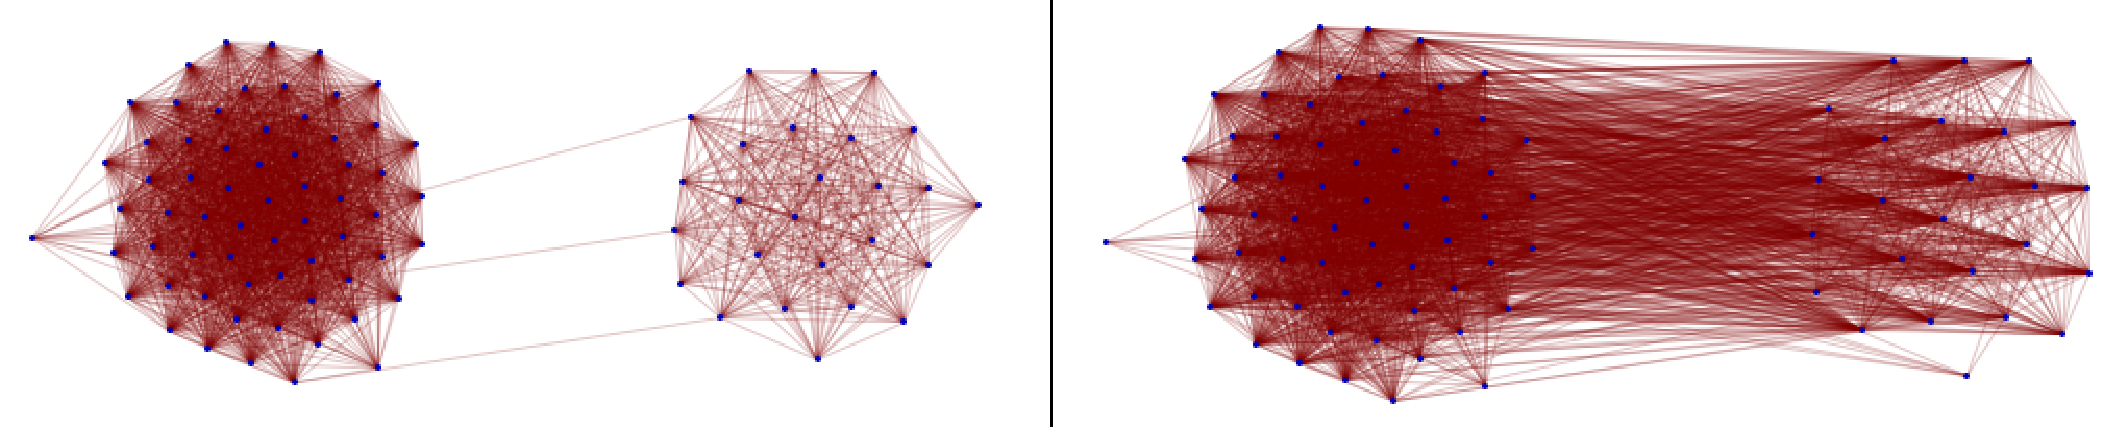
\includegraphics[width=\columnwidth]{figures/reality-mining-comparison.pdf}
%\par\end{centering}
%\caption{Left: the results of LBGA on the RealityMining dataset. Right: the
%input graph of Bluetooth scan events. LBGA was run with $consistentNO$, $\nu =
%\varepsilon = 0.2$, $\delta = 0.05$} 
%\label{fig:reality-mining-comparison}
%\end{figure}

\begin{figure}[t]
\begin{centering}
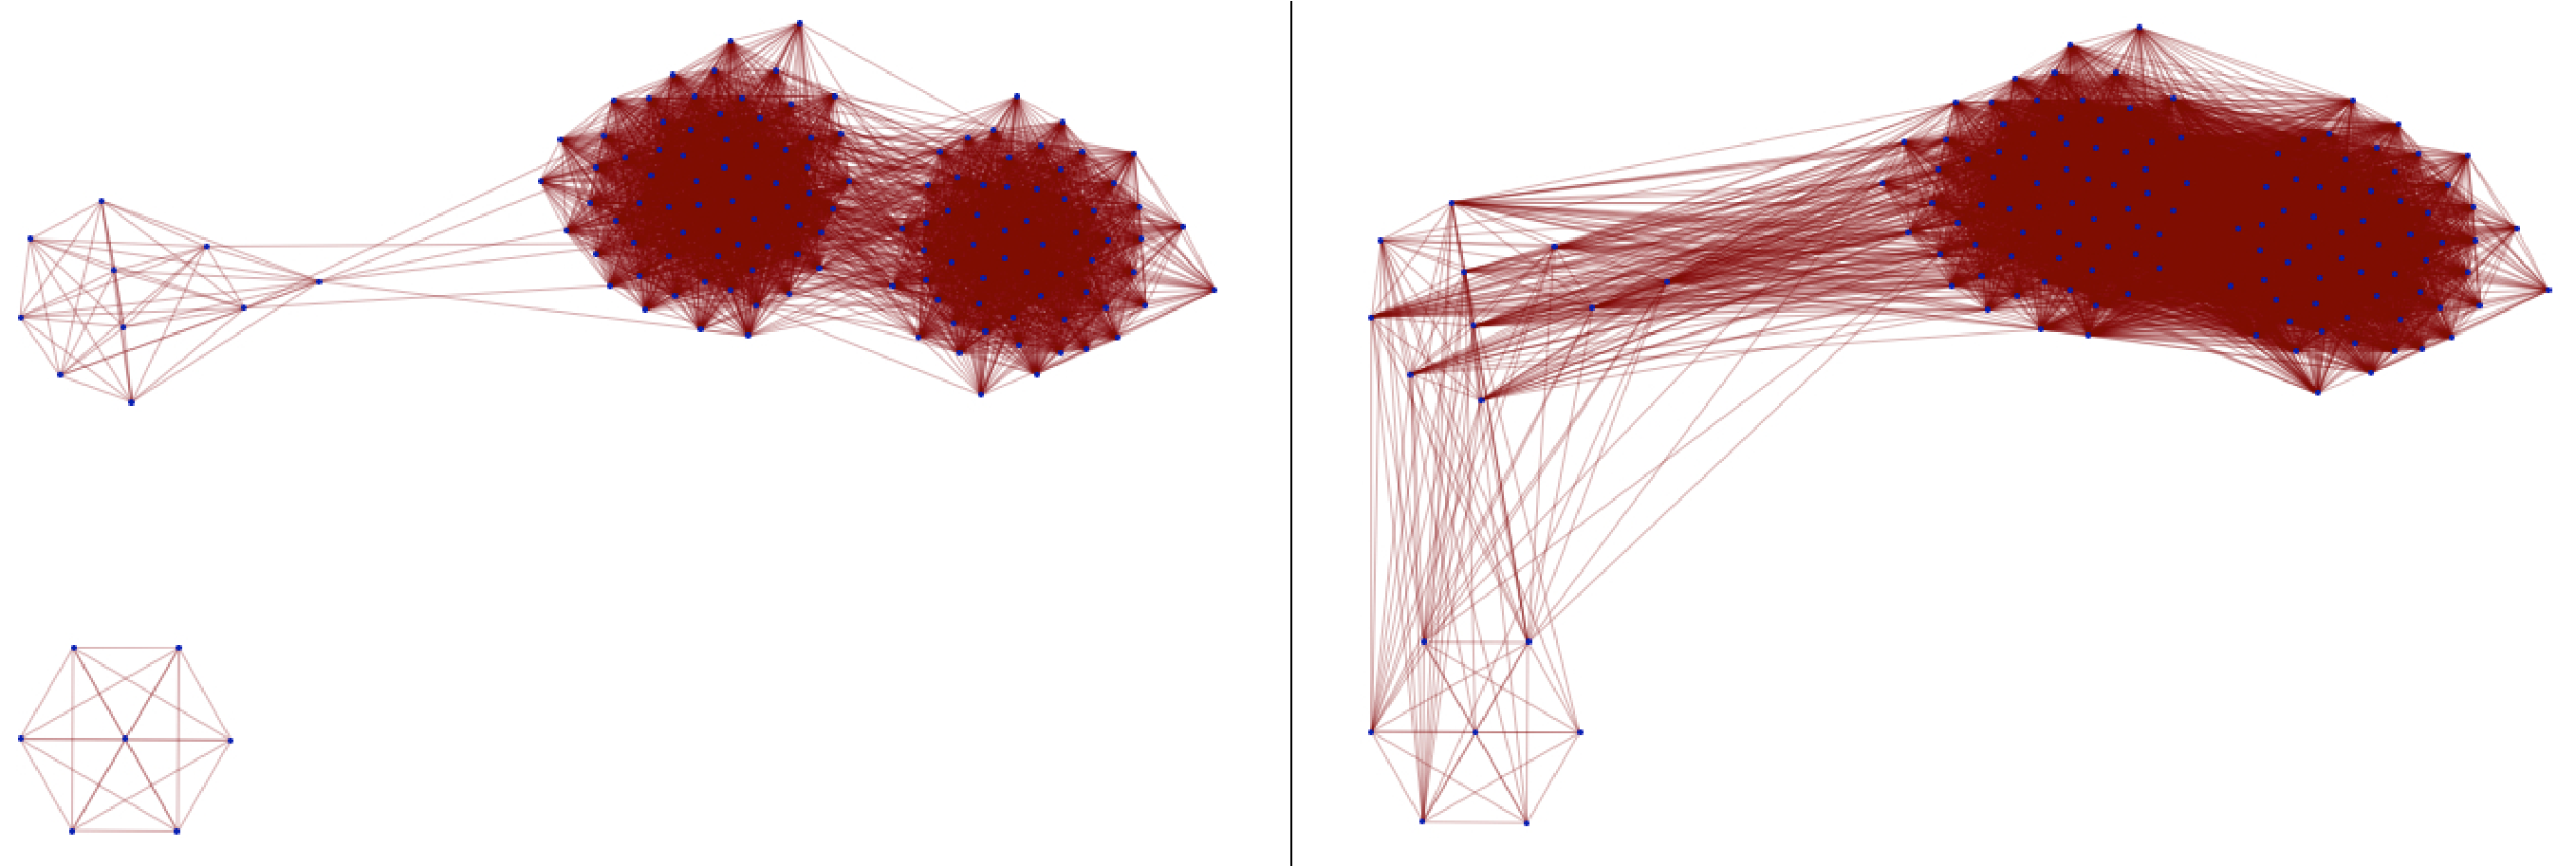
\includegraphics[width=\columnwidth]{figures/enron-comparison.pdf}
\par\end{centering}
\caption{Left: the results of LBGA on the Enron dataset. Right: the input graph
of topic models thresholded at 0.9. LBGA was run with $consistentNO$, $\nu =
\varepsilon = 0.2$, $\delta = 0.05$} 
\label{fig:enron-comparison}
\end{figure}


\subsection{Comparison with GraphFuse}
We compare LBGA with GraphFuse~\cite{Papalexakis2013}, a multi-graph clustering
algorithm that falls under the category of tensor-based clustering
~\cite{kolda2009,Tang2009}. GraphFuse computes the clustering based on
the CP decomposition of the tensor formed by appending the adjacency matrices
of the different graph sources. It differs fundamentally from LBGA in that it
does not produce an aggregated graph representation. We use NMI with the
ground truth as the performance measure. For the comparison analysis we have
only considered the synthetic datesets where the notion of ground truth is
clear and avoided the real datasets where the notion of ground truth is
subjective. Table~\ref{EC_NO} contains the comparison results. 

We find that $consistentNO$ outperforms GraphFuse on both the global block
models and the lower-noise local block models LSBM-2 and LSBM-3. LBGA also
produces very sparse representations that may be useful for future analysis,
while GraphFuse only produces a clustering.


\begin{table*}
\large
\setlength\extrarowheight{7pt}
\centering
\resizebox{\textwidth}{!}{
\begin{tabular}{| l | c c c | c | c c c  r l | c c c  r l |}
\hline 

\multicolumn{1}{| l}{} &  \multicolumn{3}{c|}{Union Graph} & \multicolumn {1} {c|}{GraphFuse} & \multicolumn{5}{c|}{LBGA: ConsistentNO}\\
\hline
Dataset  & Modularity & Conductance & NMI & NMI & Modularity & Conductance & NMI & Sparsity & Edge Type Weights \\
\hline
\hline

GSBM-4   &  0.178 &  10.678   &  1.000    &  0.716  &  0.739 &  0.084 &  1.000 &  0.433 &  (3.46,2.92,3.08,2.43)   \\
GSBM-5   &  0.093 &  15.368   &  0.636    &  0.616  &  0.727 &  2.121 &  0.619 &  0.235 &  (2.02,1.75,1.33,1.32)   \\
\hline
LSBM-1   &  0.103 &  14.725   &  0.724    &  0.686  &  0.568 &  3.322 &  0.536 &  0.274 &  (1.86,1.91,1.87,1.92)   \\
LSBM-2   &  0.166 &  11.233   &  0.992    &  0.760  &  0.740 &  0.084 &  0.992 &  0.420 &  (3.01,2.89,3.04,2.98)   \\
LSBM-3   &  0.166 &  11.216   &  1.000    &  0.779  &  0.737 &  0.104 &  1.000 &  0.422 &  (2.99,3.01,2.95,2.97)   \\

\hline
ER only  & -0.002 & 24.729    &  -        & -       &  0.193 & 112.947 & -    &  0.230  & (0.251,0.253,0.248,0.247)\\
\hline
DBLP     & 0.386  & 1368.859  &  -        & -       &  0.695 & 159.286 & -    &  0.632  & (0.432,0.568)\\
RealityMining & 0.452 & 70.314 &   -      & -       &  0.246 & 0       & -    &  0.646  & (0.365,0.091,0.198,0.115,0.115,0.115) \\
Enron  & 0.559 & 134.572 &  -   & - &   0.444  & 0.594 & -   &  0.631    & (0.390,0.610)\\
\hline
\end{tabular}
}
\caption{LBGA performance results, compared to GraphFuse and a baseline union
aggregation. All datasets in this table were run with $consistentNO$ using
$\varepsilon = \nu = 0.2, \delta = 0.05$. Union modularity and conductance for
real datasets was computed with the walktrap clustering. The order of edge type
weights for the real datasets are: DBLP (coauthorship, title similarity);
RealityMining (bluetooth, phone calls, cell tower proximity, reported
friendship, in-lab proximity, out-lab proximity); Enron (email, topic
similarity).} 
\label{EC_NO}
\end{table*}



\section{Robustness and scaling}
\label{sec:additional-analysis}

\subsection{LBGA does not boost noise}\label{sec:boostnoise} We consider
whether LBGA falsely boosts noise to ``find'' community structure where none is
present. While this depends crucially on the choice of quality function and
event, we find that for $consistentNO$ and walktrap clustering LBGA does not
falsely boost noise. Indeed, we even claim that LBGA recovers from initially
poor luck, which agrees with the theoretical adversarial bandit foundations. As
evidence we consider Figures~\ref{fig:local-sbm} and~\ref{fig:eronly}, which
respectively depict the behavior of LBGA on a local stochastic block model with
an extra \er graph and a dataset comprised entirely of \er random graphs. The
assumption is that \er graphs have no community structure.

In Figure~\ref{fig:local-sbm} we see that initially LBGA weights the \er graph
(the pink line) higher than the graphs from the LSBM model, but by round 300 it
has recovered and ultimately produces the ground truth clustering. In
Figure~\ref{fig:eronly} we see that LBGA produces aggregate graphs whose maximal
modularity values and minimum conductance values are poor, and the final
representation is very sparse. In both of these cases we see that LBGA largely
discards noise. 

Finally, we observe the phase transition for a dataset of \er random graphs (on
$n=500$ vertices) as the probability of an edge increases in
Figure~\ref{fig:erpvaries}. We see a clear phase transition around $p = 0.3$,
before which modularity values are low and conductance values are high. This
provides evidence that LBGA with consistentNO does not falsely boost sparse
amounts of noise, but will err on datasets with very high levels of noise.




\subsection{Sensitivity analysis} \label{sec:sensitivity-analysis} We analyze
the sensitivity of LBGA to noise. In Figure~\ref{fig:sensitivity-analysis} we
display performance as measured by NMI when the graph inputs are LSBM models
across different intra-cluster probability values $p_i$ and varying SNR values.
We make the following general observations.  The algorithm is consistent in
that as the noise rate $r_i$ increases, the NMI values do deteriorate as
expected. The algorithm both reaches higher quality and maintains the quality
longer for denser graphs, which again is consistent with our expectations. At a
signal to noise ratio of 2 or less, the NMI is bad for $consistentNO$ and all
choices of $p_i$. The sharp drop in quality is related to the well-known  phase
transition in the community detection problem \cite{nadakuditi2012}.
Therefore, the distance from the theoretical detectability bound on community
detection could be used as an agnostic measure to gauge the usefulness of LBGA
with a particular quality metric.


\begin{figure}[bht]
\includegraphics[scale=0.7]{figures/signal-to-noise-consistentNO.pdf}
\caption{Performance of LBGA (measured by NMI) as a function of SNR for the
LSBM model with different probabilities $p_i$ for $consistentNO$.} 
\label{fig:sensitivity-analysis}
\end{figure}

\subsection{Scalability analysis}
\label{sec:scalability-analysis}

We run a larger version of the LSBM-2 model ($m=k=10,p_i=0.3,r_i=0.05$) to
illustrate how LBGA scales for larger graphs. As shown in
Figure~\ref{fig:scalability-analysis}, LBGA scales linearly with the number of
edges. Given that real-world graphs are usually sparse, this scaling behavior
makes LBGA computationally suitable for large graphs.

LBGA was designed and implemented with scaling in mind, and the process of
fixing vertex-pairs as they are learned is largely the reason for the nice
scaling properties of Algorithm~\ref{alg:nef}. Moreover, the parameter $\delta$
encapsulates a trade-off between runtime and accuracy. Should linear scaling be
insufficient, LBGA's design allows for additional modifications to improve
scalability.  For example: quality functions that are sufficiently local allow
one to parallelize the weight update step; one could sample a sublinear number
of edges in each round and only update weights within the subgraph; one might
specify a set of ``seeds'' (vertices of interest), and sample edges local to
those vertices. While these methods are currently just potential directions for
future work, there is clearly much potential for further improvements of LBGA's
computational efficiency.

\begin{figure}[bht]
\begin{centering}
\scalebox{0.6}{\includegraphics{figures/lbga-scalability-edges.pdf}}
\par\end{centering}
\caption{The runtime of LBGA.} 
\label{fig:scalability-analysis}
\end{figure}


\section{A convergence theorem}
\label{sec:convergence-theorem}

In this section we provide a theorem on the convergence rate of LBGA. The
result can be interpreted as follows: if the quality function is sufficiently
knowledgeable about the application domain, then LBGA will converge to the
``right'' graph representation. Specifically, we assume the quality function
$q$ is a probabilistic oracle for the ground-truth clustering, which can be
interpreted as a local weak learner.  

We first set up some notation. Let $H_1, \dots, H_N$ be graphs on the same
vertex set $V$. Let $G^*$ be a target graph. For clustering we assume $G^*$ is
a disjoint union of the clusters, but the theorem applies to any target graph.
Call a graph $H_i$ \emph{good} for a vertex pair $(u,v)$ if $(u,v)$ is an edge
of both $H_i$ and $G^*$, or $(u,v)$ is an edge of neither $H_i$ nor $G^*$.
Otherwise call $H_i$ \emph{bad} for $(u,v)$. For $0 \leq \eta < 1/2$ define the
\emph{noisy oracle} $Q_\eta$ so that $Q_\eta$ is correct with probability $1/2
+ \eta$ and incorrect with probability $1/2 - \eta$. In formulas,
\[
   \begin{aligned}
   \Pr[Q_\eta(u,v) = 1  \mid (u,v) \in E(G^*)]      &= \frac{1}{2} + \eta, \\ 
   \Pr[Q_\eta(u,v) = -1 \mid (u,v) \in E(G^*)]      &= \frac{1}{2} - \eta, \\ 
   \Pr[Q_\eta(u,v) = 1  \mid (u,v) \not \in E(G^*)] &= \frac{1}{2} - \eta,\\
   \Pr[Q_\eta(u,v) = -1 \mid (u,v) \not \in E(G^*)] &= \frac{1}{2} + \eta.
   \end{aligned}
\]
The multiplicative update for good graphs is the opposite of that for bad
graphs (regardless of the value of $Q_\eta$). Thus, we can remove the
conditioning, and define $q_\eta$ to be a $\{ -1 , 1 \}$-valued random variable
which is 1 with probability $1/2 + \eta$. Without loss of generality, the
update rule in LBGA can be expressed by the multiplicative factor of $(1 +
q_{\eta} \varepsilon)$ for good graphs and $(1 - q_\eta \varepsilon)$ for bad
graphs. Further note that $\mathbb{E}[q_\eta] = 2\eta$ for good graphs and
$-2\eta$ for bad graphs.

Fix a vertex pair $(u,v)$. Let $w_{u,v,i}$ be the weight of $(u,v)$  with
respect to $H_i$.  Define $w_{u,v,\textup{good}} = \sum_{\textup{good } H_i}
w_i$ to be the sum of the weights of the good graphs for $(u,v)$, and
$w_{u,v,\textup{bad}} = \sum_{\textup{bad } H_i} w_i$ the sum of the bad
weights. Call $p_{u,v,\textup{good}}, p_{u,v,\textup{bad}}$ the corresponding
probability weights of picking a good or bad input graph. When $u,v$ are clear
from the context, we will omit them from the subscripts and simply write
$w_{\textup{good}}$, etc. We add a superscript $t$ to any quantity that changes
over rounds to denote which round of LBGA the quantity refers to. Our goal is
to bound $p_{\textup{bad}}^t$ for $t = O(\log(1/ \delta))$. Denote by
$m_{\textup{bad}} = w_{\textup{bad}}^1, m_{\textup{good}} =
w^1_{\textup{good}}$, the number of bad and good input graphs, respectively,
with $m = m_{\textup{bad}} + m_{\textup{good}}$. 


\begin{thm}

Set $\nu = \varepsilon < 1/2$ and $\eta < 1/2$ such that $0 < \varepsilon <
4\eta$.  Fix a vertex pair $(u,v)$ and assume $m_{u,v,\text{good}} \geq 1$.
Then for any $0 < \delta < 1$ and $0 < s < 1$, after $O(\log(1 / \delta) +
\log(1/s) + \log(m))$ rounds, the value $p_{u,v,\text{bad}}^t < \delta$ with
probability at least $1-s$.  \label{thm:probabilistic-oracle} 

\end{thm}


\begin{IEEEproof}
Call $q_i$ a sequence of random variables that are independent and identically
distributed according to $q_\eta$. It follows from our observations in defining
$q_\eta$ and simple induction that 
$$ 
   \begin{aligned}
      w_{\text{good}}^t &= m_{\text{good}} \prod_{i=1}^{t-1}(1 + q_i \varepsilon), \\ 
      w_{\text{bad}}^t &= m_{\text{bad}} \prod_{i=1}^{t-1}(1 - q_i \varepsilon).
   \end{aligned}
$$ 
By the linearity of expectation we have $ \mathbb{E}[w_{\text{good}}^t] =
m_{\text{good}} (1 + 2 \eta \varepsilon)^{t-1}; \mathbb{E}[w_{\text{bad}}^t] =
m_{\text{bad}} (1 - 2 \eta \varepsilon)^{t-1} $, and noting $q_\eta^2 = 1$, a
standard computation provides the variance: 
$$
    \text{Var}(w_{bad}^t) = m_{\text{bad}}^2 [(1 - 4 \eta \varepsilon +
\varepsilon^2)^{t-1} - (1 - 4 \eta \varepsilon + 4 \eta^2 \varepsilon^2)^{t-1}].
$$
Note that as $\eta \to 0$ the variance tends to infinity. Next, we wish to
bound the variance uniformly in $t$. This requires that $\varepsilon < 4 \eta$,
and in that case $ \text{Var}(w_{bad}^t) \leq m_{\text{bad}}^2 (1 - 4\eta
\varepsilon + \varepsilon^2)^t $. Applying Chebyshev's inequality, we get a
bound on the magnitude of $w_{\text{bad}}^t$, namely $\Pr(w_{\text{bad}}^t > 2)
\leq \text{Var}(w_{\text{bad}}^t)$, and running LBGA for $t = O(\log(1/s))$
rounds ensures this. Indeed, to bound $
    m_{\text{bad}}^2(1 - 4 \eta \varepsilon + \varepsilon^2)^t \leq s
$ we choose
$$
    t \geq \frac{2\log(m_{\text{bad}}) + \log \left ( \frac{1}{s} \right
)}{\log \left ( 1 - 4 \eta \varepsilon + \varepsilon^2 \right )}.
$$
Note that the denominator is nonnegative, and tends to zero as $\eta \to
\varepsilon/4$. A similar analysis for $w_{\text{good}}^t$ gives
$$
        \Pr(w_{\text{good}}^t < \mathbb{E}(w^t_{\text{good}}) - 1) \leq m_{\text{good}}^2(1 + 4\eta \varepsilon + \varepsilon^2)^{t-1},
$$
and ensuring this is at most $s$ requires
$$
    t \geq \frac{2\log(m_{\text{good}}) + \log \left ( \frac{1}{s} \right
)}{\log \left ( 1 + 4 \eta \varepsilon + \varepsilon^2 \right )}.
$$
Letting $t$ be at least the maximum of these two quantities, we have that with probability at least $1-s$,
$$
    p_{\text{bad}}^t = \frac{w_{\text{bad}}^t}{w_{\text{bad}}^t +
w_{\text{good}}^t} \leq \frac{2}{m_{\text{good}}^2 (1 + 4\eta \varepsilon +
\varepsilon^2)^t}.
$$
And to ensure this is at most $\delta$ we need at least
$$
    t \geq \frac{1 + \log(1/\delta) - 2 \log(m_{\text{good}})}{\log(1 + 4\eta
\varepsilon + \varepsilon^2)}.
$$
So we pick $t$ to be at least the maximum of all three of these lower bounds,
and the proposition follows.
\end{IEEEproof}

\begin{cor}
\label{cor:probabilistic-cor}
Let $0 < \eta < 1/2$ and set $0 < \varepsilon < 4\eta$. Let $n$ be the number
of vertices of the input graphs, and suppose the number of input graphs $m$ is
$O(1)$. Suppose LBGA uses the quality function $q_\eta$, a null event $A$, and
parameters $\nu = \varepsilon$. Suppose further that for every vertex pair
$(u,v)$ some input graph $H_i$ is good for $(u,v)$.  Then for any $0 < \delta <
1$, and any $0 < s < 1$, after $O(\log(n) + \log(1/s) + \log(1/\delta))$ rounds
all $u,v$ will satisfy $p_{u,v, \text{bad}} < \delta$ with probability at least
$1-s$.
\end{cor}

\begin{IEEEproof}
Set $s' = s/n^2$. Run LBGA for $t = O(\log(1/s') + \log(1/\delta))$ rounds and
apply the union bound over edges with Theorem \ref{thm:probabilistic-oracle}.
\end{IEEEproof}

One can further prove that for sparse noise, the neighborhood overlap function
is a probabilistic oracle for the local stochastic block model. These theorems
ignore the event $A$, and the end goal of this line of inquiry would
characterize how a suitable event $A$ can compensate for increasingly weak $q$
and unreliable input graphs, since this is the real-world scenario for which we
posit LBGA is useful. This is an area for future work.

\section{Conclusions}
\label{sec:conclusion}
We present the Locally Boosted Graph Aggregation framework, a general framework
for learning graph representations with respect to an application. In this
paper, we demonstrate the strength of the framework with the application of
community detection, and we believe the framework can be adapted to other
inference goals in graphs such as link prediction or diffusion estimation. 

Our framework offers a flexible, local weighting and aggregation of different
edge sources in order to better represent the variability of relational
structure observed in real networks. Inspired by concepts in boosting and
bandit learning approaches, LBGA is designed to handle aggregations of noisy
and disparate data sources, therefore marking a departure from methods that
assume overlap and usefulness among all data sources considered. 

LBGA also simplifies the task of designing a graph aggregation algorithm into
designing a principled quality measure $q$ and global event $A$. Doing so
allows us to connect the utility of the graph representation to the application
of interest. As a byproduct, we conjecture that statistics produced by LBGA
provide information about the utility of the graph source, such as the level of
noise. Such information can be used to improve the data collection process and
partially mitigate the effects noise before it propagates to subsequent
analysis. We gave evidence for the resistance of our framework to noise by
running it on datasets with various known levels of noise, and observed the
resulting matching weight distributions. 

A primary direction for future work is to analyze the utility of our
framework with respect to other graph applications, as well as to present a
comparison of LBGA with other existing multigraph clustering
algorithms. 
%We believe link prediction and label propagation to be ripe
%candidates, and there is an established similarity metric for the former of
%Adamic and Adar\cite{Adamic01}. Our preliminary experiments have shown
%qualitatively different graph structure when using Adamic/Adar in place of
%$consistentNO$, but further research is necessary to fully understand the reason
%for it, and whether it corresponds to a qualitatively better analysis (in light
%of the wealth of literature on metrics for link prediction, we conjecture that
%it does).\footnote{There is also a technical barrier to using Adamic/Adar
%directly, it is not a [0,1]-valued function.}
Additional directions include a more thorough stability analysis of LBGA,
exploring the modifications we have suggested to improve scalability, and to
prove further theoretical results as described earlier.

\section{Acknowledgements} We thank Vineet Mehta for providing us with the
Enron topic model data, and for his many helpful discussions.

\bibliographystyle{plain}
\bibliography{graphLearning}


\end{document}

